\begin{titlingpage}


    % ---------------------------------------------------- %
    % Main Info on Contents                                %
    % ---------------------------------------------------- %
    \newcommand{\infotable}{%
        \begin{tabular}{r|l}
            \textsc{\textbf{Studiengang}}
            & Elektro- und Informationstechnik \\
            [4mm]

            \textsc{\textbf{Modul}}
            & Projekt 4 \\
            [4mm]

            \textsc{\textbf{Auftraggeber}}
            & Hans Gysin \\
            [4mm]

            \textsc{\textbf{Betreuer}}
            & Matthias Meier, Pascal Schleuniger, Pascal Buchschacher, \\
            & Anita Gertiser, Bonnie Domenghino \\
            [4mm]

            \textsc{\textbf{Team}}
            & 3 \\
            [4mm]

            \textsc{\textbf{Autoren}}
            & Marcel Heymann, Noah H\"usser, Raphael Frey, Dominik Keller,  \\
            & Marco Koch, Reto Nussbaumer, Francesco Rovelli                \\
            [4mm]

            \textsc{\textbf{Datum}}
            & \today \\
            [4mm]

            \textsc{\textbf{Version}}
            & 0.1 \\
        \end{tabular}%
    }%


    % ---------------------------------------------------- %
    % Place the Background Picture and Info Table          %
    % ---------------------------------------------------- %
    \hspace{-2.54mm}
    \newlength{\logoX}
    \setlength{\logoX}{5mm}
    \newlength{\logoY}
    \setlength{\logoY}{5mm}
    \begin{tikzpicture}[remember picture, overlay]
        % ------------------------------------------------ %
        % Background Picture                               %
        % ------------------------------------------------ %
        \node[inner sep=0pt] at (current page.center) {%
            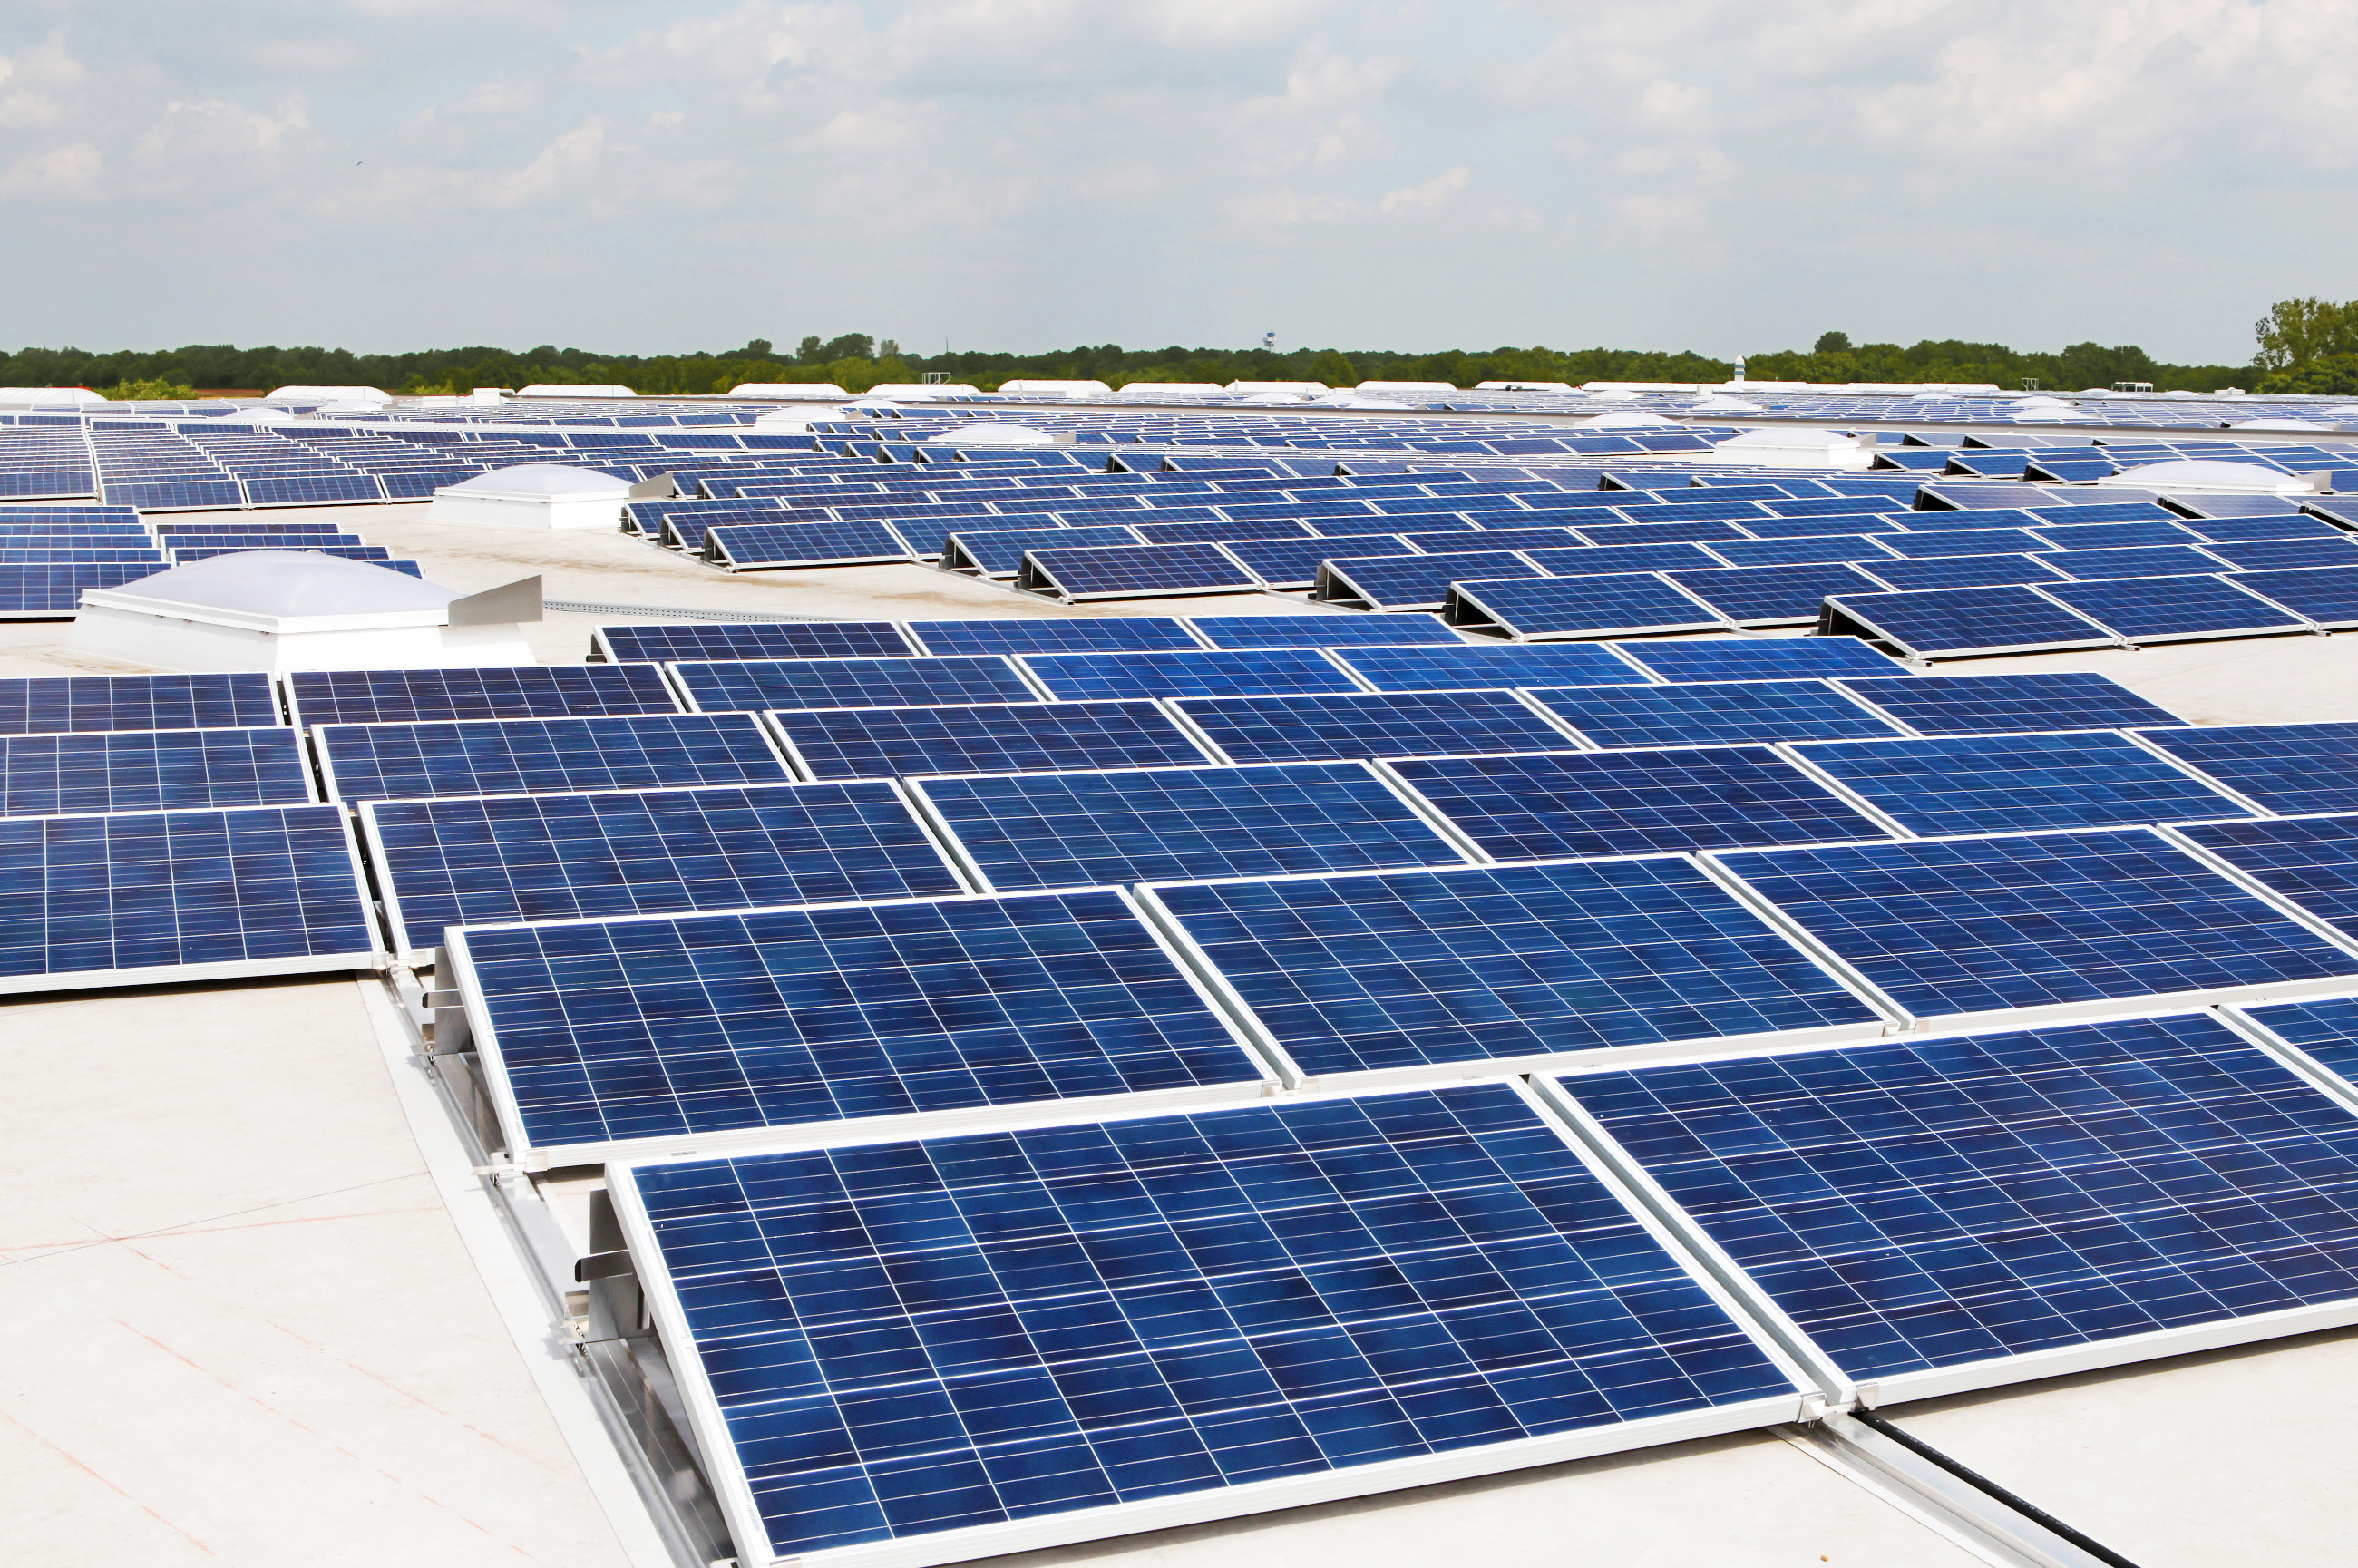
\includegraphics[width=\paperwidth,height=\paperheight]{images/titlepage/titlepic.jpg}%
        };

        % ------------------------------------------------ %
        % Info Table                                       %
        % ------------------------------------------------ %
        \node[%
            fill=black,
            fill opacity=0.75,
            rounded corners,
            outer sep=0pt,
            inner sep=1em,
            yshift=9em,
            anchor = south%
        ] at (current page.south) {\textcolor{white}{\infotable}};

        % ------------------------------------------------ %
        % FHNW Logo                                        %
        % ------------------------------------------------ %
        \node[anchor=north west,xshift=\logoX,yshift=-\logoY,outer sep=0pt,inner sep=0pt] at (current page.north west) {%
            
\includegraphics[height=12mm]{images/titlepage/fhnw.eps}%
        };
    \end{tikzpicture}



    % ---------------------------------------------------- %
    % The Text can  be set rather low in  the page without %
    % adjusting the top lengths.                           %
    % Backing up  and reseting these lengths  seems not to %
    % be necessary;  it appears  they are restored  at the %
    % end of the titlingpage environment.                  %
    % ---------------------------------------------------- %
    \setlength{\headsep}{0pt}
    \setlength{\headheight}{0pt}
    \setlength{\uppermargin}{4em}
    \checkandfixthelayout


    % ---------------------------------------------------- %
    % By   default,  centering   inside  the   titlingpage %
    % environment  will   center  with  respects   to  the %
    % typeblock. When  the  typeblock  is  centered,  this %
    % leads to  centered text  with respect to  the entire %
    % title  page. However,  When  the  typeblock  is  not %
    % centered, some adjustment is needed.                 %
    % See memman Chapter "Titles" for more information.    %
    % ---------------------------------------------------- %
    \calccentering{\unitlength}
    \begin{adjustwidth*}{\unitlength}{-\unitlength}


    % ---------------------------------------------------- %
    % Work some  magic to  automatically adjust  the hrule %
    % lengths to the length of the book title.             %
    %                                                      %
    % NOTE: The  font  size setting  needs  to  be in  the %
    % \mytitle  command, otherwise  \settolength will  not %
    % take it  into account  and will only  calculate with %
    % the default font size.                               %
    %                                                      %
    % NOTE  2: This mechanism  breaks if  the title  spans %
    % across multiple  lines. You're on  your own  in that %
    % case.                                                %
    % ---------------------------------------------------- %
    %\newcommand{\mytitle}{{\textbf{\fontsize{25mm}{1em}\selectfont Project Powerline}}} % default font
    \newcommand{\mytitle}{{\textbf{\fontsize{12mm}{1em}\selectfont Project Powerline}}}
    \newlength{\titlelength}            % Length of title text
    \settowidth{\titlelength}{\mytitle}
    \newcommand{\titlerulefactor}{1.2}  % Length of title rules, as a factor

    % ---------------------------------------------------- %
    % Set the title color                                  %
    % ---------------------------------------------------- %
    \newcommand{\titlecolor}{black}

    % ---------------------------------------------------- %
    % Put the title onto the page                          %
    % ---------------------------------------------------- %
    \textcolor{\titlecolor}{%
        \centering
        \rule{\titlerulefactor\titlelength}{1pt} \\
        \vspace*{4mm}
        \mytitle\\
        %\vspace*{5mm}
        \rule{\titlerulefactor\titlelength}{1pt} \\
        \vspace*{6mm}
        \fontsize{8mm}{1em}\selectfont Fachbericht \\
    }


    % ---------------------------------------------------- %
    % This is the end of the centering magic.              %
    % ---------------------------------------------------- %
    \end{adjustwidth*}


    % ---------------------------------------------------- %
    % Make  sure  this  is   not  put  into  \frontmatter, %
    % otherwise it will get a \frontmatter folio.          %
    % \cleardoblepage  is not  actually necessary  because %
    % it  is  automatically   called  by  the  titlingpage %
    % environment.                                         %
    % ---------------------------------------------------- %
    %\cleardoublepage

    %\setlength{\headsep}{\originallength}
    %\checkandfixthelayout
\end{titlingpage}
